\section{PREFLEX}

The \ac{PREFLEX} architecture can be split into two independent components. At the network, a mechanism for \ac{PREF} is defined, whereby stub domains can signal a preferred path to end-hosts according to local policy or perceived path quality. At the end-hosts, a transport agnostic protocol for \ac{LEX} is used, which explicitly marks packets within a flow in order to signal path loss back to the network.

While functionally separate, in practice both components work in tandem. The use of loss exposure, while executed by hosts, provides network operators with feedback on end-to-end path loss. Conversely, with path re-feedback hosts are allowed access to paths selected by the network. Together, \ac{PREFLEX} bridges the divide between network and transport layers and facilitates balancing by congestion, rather than necessarily load, over the multiple paths typically available solely to edge networks.

\subsection{Loss Exposure}

\ac{LEX} is proposed as a simple protocol for revealing loss, which not only borrows heavily from re-\ac{ECN} \cite{Briscoe:2008p494}, a protocol for congestion exposure, but which can coexist and serve as a stepping stone for the deployment of the latter. Revealing information currently confined to the transport layer down to the network both reduces the need for the network to inspect higher level protocol headers in order to redistribute bandwidth differently and corrects the information asymmetry that currently afflicts networks, who know less about the quality of service they provide than their customers.

The first change proposed for \ac{LEX} is to have end-hosts mark, at the network layer, packets belonging to flows where feedback has not been established. 
This typically corresponds to the first packet exchange in a flow, such as SYN packets in \ac{TCP}, but may also include the first packet after a significant idle period, a keep-alive packet or a renewed attempt at a retransmission after successive timeouts in the case of network failure. 
Within \ac{LEX}, as with re-\ac{ECN}, such packets are labelled \ac{FNE}.

%re-ecn uses only for policing
The signalling of such packets has many practical implications. 
For one, from simply inspecting the \ac{IP} header, networks are made aware of the first of a succession of similar packets, which poses significant advantages in allocating state in middleboxes, whether it be to perform admission control, policing or traffic shaping. 
All of the above are possible by inspecting \ac{TCP}, but this makes apparent an architectural illusion: that a connectionless layer should be oblivious to connection setup. 
Explicitly providing such information at the \ac{IP} layer alleviates in some measure the need for consistent violation of layering by network equipment, or hopefully circumscribes such practices to a small subset of packets.

Additionally, the concept of a transport flow, which establishes an association between two endpoints, is decoupled from the concept of a network flow, which will henceforth be referred to as a flowlet \cite{Sinha:2004p124}. 
A flowlet is defined as a stream of packets which end-hosts expect to follow the same network path. 
The same transport flow may be composed of a single flowlet, parallel flowlets, or a succession of different flowlets. 
This feature is particularly advantageous for balancing traffic as flowlets provide a finer granularity than existing flows, as well as allowing flows to quickly switch path without breaking the transport session.

Once feedback has been established, hosts adjust their sending rate in response to implicit congestive signals such as delay or packet loss, or explicit signals such as \ac{ECN}. Protocols for congestion exposure, such as re-\ac{ECN}, mark outgoing packets according to the explicit congestion marking received from the network. As such, \ac{IP} packets would carry two congestion markings. The first indicating the congestion experienced so far and the second indicating the end-to-end congestion experienced by the host in the previous RTT. With this re-feedback of congestion markings, networks are able to estimate rest-of-path congestion, which is an important metric for keeping customers accountable for the congestion they cause and providers accountable for the services they offer.

\ac{LEX} specifies a simplified form of congestion exposure which uses the implicit information contained in losses as opposed to relying on the widespread deployment of congestion notification. Where packet loss does arise, \ac{LEX} requires that hosts mark their respective retransmits with a \ac{LEX} code point. The drawback of this approach is that only the end-to-end congestion can be estimated from a stream of packets, which implies that traffic can only be reliably aggregated close to the source, and effectively policed close to the receiver. Since the focus of \ac{PREFLEX} is balancing congestion at a stub domain however, this limitation is not significant.

\begin{table}
\centering
\begin{tabular}{r|l}
    \textbf{Code point} & \textbf{Meaning} \\
    Not-\acs{LECT} & Not \acf{LECT} \\
    \acs{LECT} & \acf{LECT} \\
    \acs{LEX} & \acf{LEX} \\ 
    \acs{FNE} & \acf{FNE} \\
\end{tabular}
\caption{LEX code points and description.}
\label{table:codepoint}
\end{table}

If run as a complement of re-\ac{ECN}, three of the four code points in table~\ref{table:codepoint} are potentially shared, in which case only the loss experienced code point has to be added to the re-\ac{ECN} specification. For routers along the path, an accurate estimate of the end-to-end path loss can be obtained by simply dividing the sum of bytes marked with the loss experienced code point, by the total traffic marked as either \ac{LECT} or \ac{LEx}. Additionally, one could envision a preferential dropping mechanism which prioritizes retransmits.

\subsection{Path Re-feedback}

For networks, the most significant hurdle in adopting multiple paths for a single destination is not the path selection process, but rather the difficulty in assigning packets to paths. Since balancing traffic at a packet granularity has severe repercussions for the transport layer, network operators have typically resorted to splitting traffic by destination prefix. Increasingly, networks have also been able to afford the cost of keeping flow state in an attempt to balance traffic at a finer granularity. 

Neither of these approaches are strictly necessary in a mutualistic architecture. Since hosts are made aware of the path packets take, flow state can be pushed outwards, placing the responsibility for assigning packets to paths at the endpoints. In such a case, a network only needs to perform path selection according to local policy and pass the information onto the end-host.

For this purpose, \ac{FNE} packets, as defined in \ac{LEX}, are used to act as network triggers for path selection. 
An \ac{ISP} or stub domain, upon detecting an incoming \ac{FNE} packet, selects a preferred outgoing path based on the reverse lookup of the source address, and marks the packet with a path identifier. 
For \ac{IPv4}, a possible location for such marking to occur could be within the \ac{DS} field, where a set of code points are reserved for local use. 
On receiving an \ac{FNE} packet containing a path identifier, a sender should tag all subsequent packets in the flowlet using the same identifier in order to ensure it will traverse the selected egress at the edge domain.

\begin{figure}
    \begin{subfigure}[b]{0.5\textwidth}
        \centering
        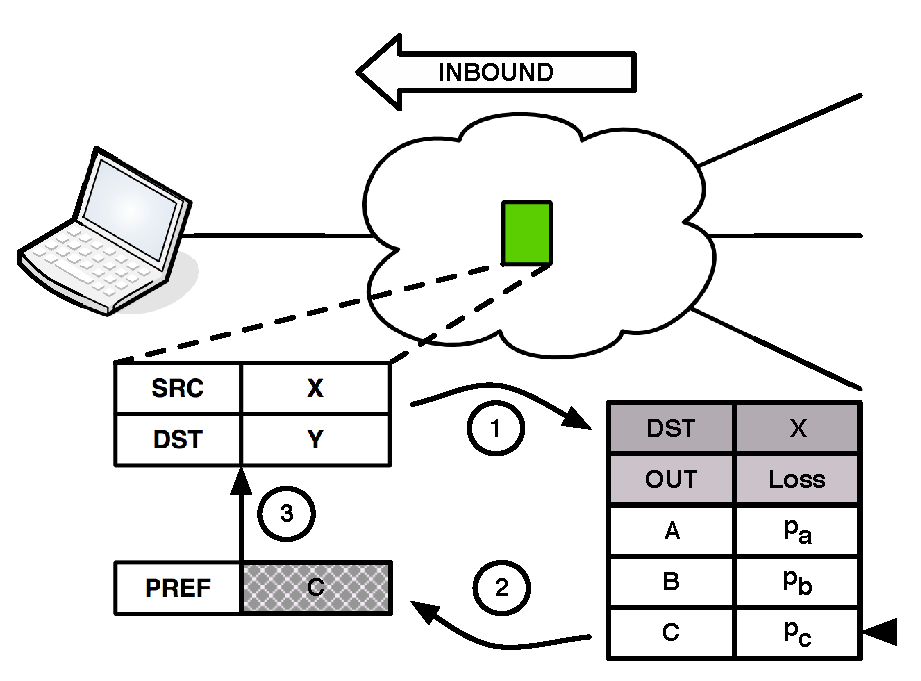
\includegraphics[width=2.5in]{figures/preflex/preflex1}
        \caption{Inbound \acs{FNE} packet}
        \label{fig:preflexin}
    \end{subfigure}%
        %add desired spacing between images, e. g. ~, \quad, \qquad etc. 
        %(or a blank line to force the subfigure onto a new line)
    \begin{subfigure}[b]{0.5\textwidth}
        \centering
        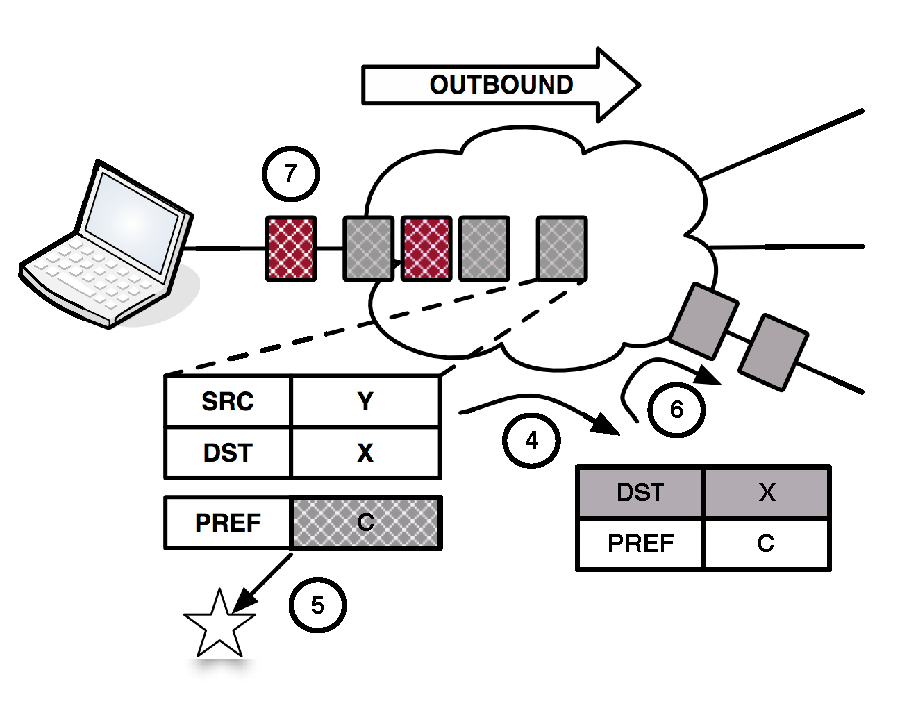
\includegraphics[width=2.5in]{figures/preflex/preflex2}
        \caption{Outbound traffic}
        \label{fig:preflexout}
    \end{subfigure}
    \caption{\acs{PREFLEX} architecture.}
    \label{fig:preflex}
\end{figure}

This behaviour is exemplified in figure \ref{fig:preflex}.  
In \ac{PREF} the network selects a preferred outgoing path for each incoming \ac{FNE} packet (figure \ref{fig:preflexin}). 
Upon receiving the first packet of a flowlet, the \ac{PREFLEX} aware router performs a reverse lookup on the source address (step 1) and selects a path according to the perceived performance (2). 
The router then associates the chosen path identifier to the packet and forwards the packet toward the host (3).
The treatment of outbound traffic by \ac{PREFLEX} is illustrated in figure \ref{fig:preflexout}. 
The host, having received indication of the preferred path, tags all traffic deemed sensitive to reordering with the given path identifier. 
As the \ac{PREFLEX} aware router receives this marked traffic it updates statistics associated to path, aggregating loss for each destination prefix (4). 
It then discards the path identifier (5) and forwards traffic along the appropriate path (6). 

A subtle implication of triggering path selection based on incoming packets, rather than resorting to out-of-band signalling for example, is that path selection becomes receiver driven. The responsibility for defining a strategy on when and how often to attempt a path request lays firmly with the stakeholder who extracts the most benefit. The flip side is that because \ac{FNE} packets require additional network intervention, whether for selecting a new path or setting up state, networks may rate limit the amount of \ac{FNE} packets they receive in order to protect themselves from overload. This is the current line of thinking with re-\ac{ECN}, where \ac{FNE} packets are used to set state in congestion policers.

